\documentclass[10pt]{article} 

\usepackage{fullpage}
\usepackage{bookmark}
\usepackage{amsmath}
\usepackage{amssymb}
\usepackage[dvipsnames]{xcolor}
\usepackage{hyperref} % for the URL
\usepackage[shortlabels]{enumitem}
\usepackage{mathtools}
\usepackage[most]{tcolorbox}
\usepackage[amsmath,standard,thmmarks]{ntheorem} 
\usepackage{physics}
\usepackage{pst-tree} % for the trees
\usepackage{verbatim} % for comments, for version control
\usepackage{tabu}
\usepackage{tikz}
\usepackage{float}

\lstnewenvironment{python}{
\lstset{frame=tb,
language=Python,
aboveskip=3mm,
belowskip=3mm,
showstringspaces=false,
columns=flexible,
basicstyle={\small\ttfamily},
numbers=none,
numberstyle=\tiny\color{Green},
keywordstyle=\color{Violet},
commentstyle=\color{Gray},
stringstyle=\color{Brown},
breaklines=true,
breakatwhitespace=true,
tabsize=2}
}
{}

\lstnewenvironment{latex}{
\lstset{
backgroundcolor=\color{white!90!NavyBlue},   % choose the background color; you must add \usepackage{color} or \usepackage{xcolor}; should come as last argument
basicstyle={\scriptsize\ttfamily},        % the size of the fonts that are used for the code
breakatwhitespace=false,         % sets if automatic breaks should only happen at whitespace
breaklines=true,                 % sets automatic line breaking
captionpos=b,                    % sets the caption-position to bottom
commentstyle=\color{Gray},    % comment style
deletekeywords={...},            % if you want to delete keywords from the given language
escapeinside={\%*}{*)},          % if you want to add LaTeX within your code
extendedchars=true,              % lets you use non-ASCII characters; for 8-bits encodings only, does not work with UTF-8
% firstnumber=1000,                % start line enumeration with line 1000
frame=single,	                   % adds a frame around the code
keepspaces=true,                 % keeps spaces in text, useful for keeping indentation of code (possibly needs columns=flexible)
keywordstyle=\color{Violet},       % keyword style
language=[latex]tex,                 % the language of the code
morekeywords={*,...},            % if you want to add more keywords to the set
% numbers=left,                    % where to put the line-numbers; possible values are (none, left, right)
% numbersep=5pt,                   % how far the line-numbers are from the code
% numberstyle=\tiny\color{Green}, % the style that is used for the line-numbers
rulecolor=\color{black},         % if not set, the frame-color may be changed on line-breaks within not-black text (e.g. comments (green here))
showspaces=false,                % show spaces everywhere adding particular underscores; it overrides 'showstringspaces'
showstringspaces=false,          % underline spaces within strings only
showtabs=false,                  % show tabs within strings adding particular underscores
stepnumber=2,                    % the step between two line-numbers. If it's 1, each line will be numbered
stringstyle=\color{Brown},     % string literal style
tabsize=2,	                   % sets default tabsize to 2 spaces
title=\lstname}                   % show the filename of files included with \lstinputlisting; also try caption instead of title
}
{}

% floor, ceiling, set
\DeclarePairedDelimiter{\ceil}{\lceil}{\rceil}
\DeclarePairedDelimiter{\floor}{\lfloor}{\rfloor}
\DeclarePairedDelimiter{\set}{\lbrace}{\rbrace}
\DeclarePairedDelimiter{\iprod}{\langle}{\rangle}

\DeclareMathOperator{\Int}{int}
\DeclareMathOperator{\mean}{mean}

% commonly used sets
\newcommand{\R}{\mathbb{R}}
\newcommand{\N}{\mathbb{N}}
\newcommand{\Q}{\mathbb{Q}}
\renewcommand{\P}{\mathbb{P}}

\newcommand{\sset}{\subseteq}

\theoremstyle{break}
\theorembodyfont{\upshape}

\newtheorem{thm}{Theorem}[subsection]
\tcolorboxenvironment{thm}{
enhanced jigsaw,
colframe=Dandelion,
colback=White!90!Dandelion,
drop fuzzy shadow east,
rightrule=2mm,
sharp corners,
before skip=10pt,after skip=10pt
}

\newtheorem{cor}{Corollary}[thm]
\tcolorboxenvironment{cor}{
boxrule=0pt,
boxsep=0pt,
colback={White!90!RoyalPurple},
enhanced jigsaw,
borderline west={2pt}{0pt}{RoyalPurple},
sharp corners,
before skip=10pt,
after skip=10pt,
breakable
}

\newtheorem{lem}[thm]{Lemma}
\tcolorboxenvironment{lem}{
enhanced jigsaw,
colframe=Red,
colback={White!95!Red},
rightrule=2mm,
sharp corners,
before skip=10pt,after skip=10pt
}

\newtheorem{ex}[thm]{Example}
\tcolorboxenvironment{ex}{% from ntheorem
blanker,left=5mm,
sharp corners,
before skip=10pt,after skip=10pt,
borderline west={2pt}{0pt}{Gray}
}

\newtheorem*{pf}{Proof}
\tcolorboxenvironment{pf}{% from ntheorem
breakable,blanker,left=5mm,
sharp corners,
before skip=10pt,after skip=10pt,
borderline west={2pt}{0pt}{NavyBlue!80!white}
}

\newtheorem{defn}{Definition}[subsection]
\tcolorboxenvironment{defn}{
enhanced jigsaw,
colframe=Cerulean,
colback=White!90!Cerulean,
drop fuzzy shadow east,
rightrule=2mm,
sharp corners,
before skip=10pt,after skip=10pt
}

\newtheorem{prop}[thm]{Proposition}
\tcolorboxenvironment{prop}{
boxrule=0pt,
boxsep=0pt,
colback={White!90!Green},
enhanced jigsaw,
borderline west={2pt}{0pt}{Green},
sharp corners,
before skip=10pt,
after skip=10pt,
breakable
}

\setlength\parindent{0pt}
\setlength{\parskip}{2pt}


\begin{document}
\let\ref\Cref

\title{\bf{A Tiktz Tutorial}}
\date{\today}
\author{Felix Zhou}

\maketitle
\newpage
\tableofcontents
\listoffigures
\listoftables
\newpage

\section*{Introduction}
\subsection*{What it this?}
I am an upcoming third year (3A) student at the University of Waterloo who plans to take CO342 - Introduction to Graph Theory, in Fall 2019.
To aid me and other students such as myself with typesetting graphs using tikz, I created this shortened tutorial from the TikZ and PGF Manual.
Please do not hesitate to reach out to me if there are any errors and I will publish an updated version ASAP.

\subsection*{Goal}
I have always believed in understanding your tools completely before using them.
In addition to my tutorial on TikZ, I will include as much notes on the math behind non-trivial TikZ commands as I can, with the condition that I myself at least understand the gist of the technologies.
If it is completey above me and looks like gobly goop, I will clearly note this and invite \textit{you} to write me a short section based on your understanding.


\newpage
\section{Generic Setup}
\begin{latex}
    \documentclass{article}
    \usepackage{tikz}
    \usepackage{float}

    \begin{document}
    \begin{figure}[H] % forces position of tikz to be where it is in source file
        \centering

        \begin{tikzpicture}
            % insert provided code
        \end{tikzpicture}

        \caption{A Caption}
        \label{fig:alabel}
    \end{figure}
    \end{document}
\end{latex}

This is our default setup for any document classes involving TikZ.
If additional imports are necessary, we will explicityly note them.

Note that we may ommit typing ``tikzpicture'' everytime and inline simple TikZ pictures with the ``tikz'' command.
When we do this, we will explicitly type out ``tikz``.

If an option is enabled for the entire tikzpicture environment, we will include the begin and end keywords explicitly.

\newpage
\section{Paths}

\subsection{Straight Paths}
\begin{figure}[H]
    \centering
    \begin{tikzpicture}
        \draw (-1.5,0) -- (1.5,0);
        \draw (0,-1.5) -- (0,1.5);
    \end{tikzpicture}.
    \caption{Basic Straight Path}
    \label{fig:basicstraightpath}
\end{figure}

\begin{latex}
    \draw (-1.5,0) -- (1.5,0); % draw straight lines between two points
    \draw (0,-1.5) -- (0,1.5);
\end{latex}

We can also directly inline a similar picture
\begin{figure}[H]
    \centering
    \tikz \draw (-1.5,0) -- (1.5,0) -- (0,-1.5) -- (0,1.5);
    \caption{Inlined Straight Path}
    \label{fig:inlinedstraightpath}
\end{figure}

\begin{latex}
    \tikz \draw (-1.5,0) -- (1.5,0) -- (0,-1.5) -- (0,1.5);
\end{latex}

\subsection{Curved Paths}
TikZ allows us to define arbitrary curves using control points.
The basis behind of this concept are B\'ezier Curves, which in turn are based on the Bernstein Polynomial.

\begin{figure}[H]
    \centering
    \begin{tikzpicture}
        \filldraw [gray]
        (0,0) circle (2pt)
        (1,1) circle (2pt)
        (3,3) circle (2pt)
        (3,0) circle (2pt);
        \draw (0,0) .. controls (1,1) and (3,3) .. (3,0);
    \end{tikzpicture}
    \caption{Basic Curve}
    \label{fig:basiccurve}
\end{figure}

\begin{latex}
    \filldraw [gray]
    (0,0) circle (2pt)
    (1,1) circle (2pt)
    (3,3) circle (2pt)
    (3,0) circle (2pt);
    \draw (0,0) .. controls (1,1) and (3,3) .. (3,0);
\end{latex}

The above shows a basic curve where the control points are explicitly drawn as well.
Obviously, this would be ommited (on your graph theory course home work for example).

\subsubsection{Bezier Curves and the Bernstein Polynomial}
This section gives some mathematical background on curved paths and is skippable.

\begin{defn}[B\'ezier Curve]
   A recursive definition for the B\'ezier curve of degree $n$ expresses it as a point-to-point linear combination (interpolation) of a pair of corresponding points in two B\'ezier curves of degree $n-1$.

   \begin{align*}
       B &: \R \to \R \\
       B_{P_0}(t) &= P_0 &&\text{base case} \\
       B(t) &= B_{P_0P_1\dots P_n}(t) = (1-t)B_{P_0P_1\dots P_{n-1}}(t) + tB_{P_1P_2\dots P_n}(t)
   \end{align*}
\end{defn}

\begin{defn}[Bernstein Basis Polynomials]
    of degree $n$ are given by
    \[
    \set*{b_{i, n}(t) = \binom{n}{i} t^i (1-t)^{n-i} : 0\leq i\leq n}
    \]

    which form a basis of polynomials with degree at most $n$.
\end{defn}

\begin{prop}
    \[
    B(t) = \sum_{i=0}^n \binom{n}{i} t^i(1-t)^{n-i} P_i
    \]

    So we can express a B\'ezier curve as a linear combination of the Berstein Basis.
\end{prop}

The points $P_i$ are called \textit{Control Points} for the B\'ezier Curve.
The polygon formed by connecting the B\'ezier points with lines, starting with $P_0$ and finishing with $P_n$, gives the \textit{B\'ezier Polygon (Control Polygon)}.
The convex hull of the B\'ezier Polygon contains the B\'ezier Curve.

\subsection{Circular Paths}
Although it would certainly be possible to draw all our circular paths with control points, it would prove tedious to say the least.

\begin{figure}[H]
    \centering
    \tikz \draw (0,0) circle (30pt);
    \caption{Basic Circle}
    \label{fig:basiccircle}
\end{figure}

\begin{latex}
    \tikz \draw (0,0) circle (2);
\end{latex}

We can also draw Ellipses.

\begin{figure}[H]
    \centering
    \tikz \draw (0,0) ellipse (2 and 1);
    \caption{Basic Ellipse}
    \label{fig:basicellipse}
\end{figure}

\begin{latex}
    \tikz \draw (0,0) ellipse (2 and 1);
\end{latex}

Although it is possible to draw ellipses which are rotated in arbitrary directions, we will leave this for the section on transformations later on.

\subsection{Rectangular Paths}
\begin{figure}[H]
    \centering
    \tikz \draw (0,0) rectangle (4, 3);
    \caption{Basic Rectangle}
    \label{fig:basicrectangle}
\end{figure}

\begin{latex}
    \tikz \draw (0,0) rectangle (4, 3);
\end{latex}

\subsection{Grid Paths}
\begin{figure}[H]
    \centering
    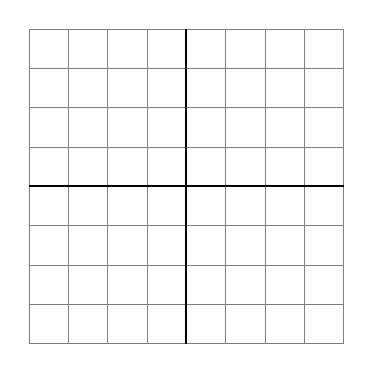
\begin{tikzpicture}
        \draw[step=.5, gray, very thin] (-2,-2) grid (2, 2);
        \draw[thick] (-2, 0) -- (2, 0);
        \draw[thick] (0, -2) -- (0, 2);
    \end{tikzpicture}
    \caption{Basic Grid}
    \label{fig:basicgrid}
\end{figure}

\begin{latex}
    \draw[step=.5, gray, very thin] (-2,-2) grid (2, 2);
    \draw[thick] (-2, 0) -- (2, 0);
    \draw[thick] (0, -2) -- (0, 2);
\end{latex}

Note how we indicated the step and, color, and thickness of the paths to TikZ to accentuate the x, y-axis instead of the entire grid.

\subsection{Arc Paths}
What if we only wish to draw part of a circle of ellipse?
TikZ has us covered.
The second argument to the arc command consists of the form (initial angle:final angle:radius/radii), where the angles are given in degrees and interpreted in a counter clockwise fashion, not unlike the unit circle and the sinusoidal functions.

\begin{figure}[H]
    \centering
    \tikz \draw (0, 0) arc (0:90:1);
    \caption{Basic Circle Arc}
    \label{fig:basiccirclearc}
\end{figure}

\begin{latex}
    \tikz \draw (0, 0) arc (0:90:1);
\end{latex}

We can actually give TWO arguments to the third parameter of the second argument to arc, which will draw an ellipse.

\begin{figure}[H]
    \centering
    \tikz \draw (0, 0) arc (0:270:1 and 2);
    \caption{Basic Ellipse Arc}
    \label{fig:basicellipsearc}
\end{figure}

\begin{latex}
    \tikz \draw (0, 0) arc (0:270:1 and 2);
\end{latex}

\subsection{Clipping}
\begin{figure}[H]
    \centering
    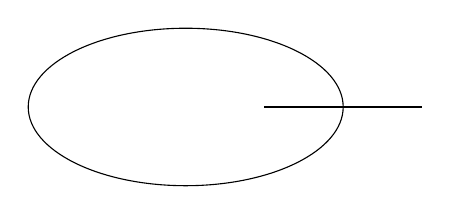
\begin{tikzpicture}
        \draw (1, 0) arc (0:360:2 and 1);
        \draw (0, 0) -- (2, 0);
    \end{tikzpicture}
    \caption{Arc Line Intersection}
    \label{fig:arclineintersection}
\end{figure}

\begin{latex}
    \draw (1, 0) arc (0:360:2 and 1);
    \draw (0, 0) -- (2, 0);    
\end{latex}

Consider the above.
Suppose we wish to emphasize the point of intersection of the arc and the line.

We can use the ``clip'' command to crop the rendering.

\begin{figure}[H]
    \centering
    \begin{tikzpicture}[scale=3]
        \clip (0.5, -0.5) rectangle (1.5, 0.5);
        \draw (1, 0) arc (0:360:2 and 1);
        \draw (0, 0) -- (2, 0);
    \end{tikzpicture}
    \caption{Rectangular Clip}
    \label{fig:rectangularclip}
\end{figure}

\begin{latex}
    \begin{tikzpicture}[scale=3]
        \clip (0.5, -0.5) rectangle (1.5, 0.5);
        \draw (1, 0) arc (0:360:2 and 1);
        \draw (0, 0) -- (2, 0);
    \end{tikzpicture}
\end{latex}

However, we are not just limited to rectangular clips!
Below shows the example above with some augmentations, an ellipse-shaped clif, as well as grid lines added.

\begin{figure}[H]
    \centering
    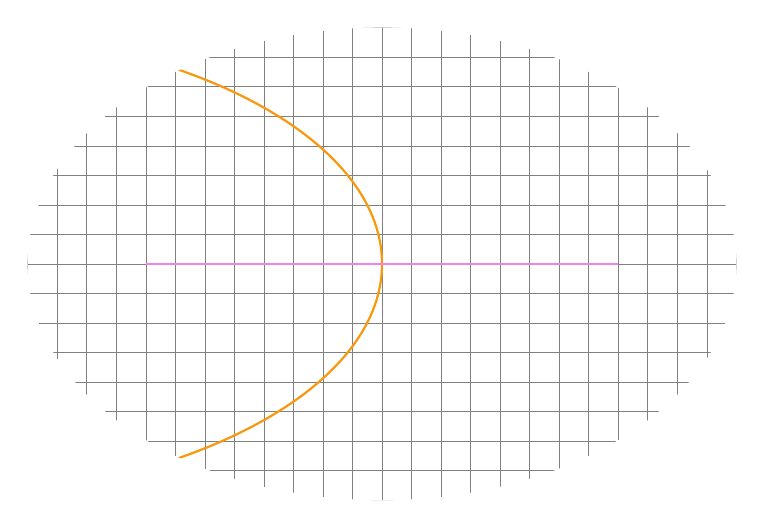
\begin{tikzpicture}[scale=3]
        \clip (1, 0) ellipse (1.5 and 1);
        \draw[step=.125, very thin, gray] (-2, -2) grid (3, 2);
        \draw[thick, color=YellowOrange] (-1, -1) arc (-90:90:2 and 1);
        \draw[thick, color=Violet] (0, 0) -- (2, 0);
    \end{tikzpicture}
    \caption{Ellipse Clip}
    \label{fig:ellpiseclip}
\end{figure}

\begin{latex}
    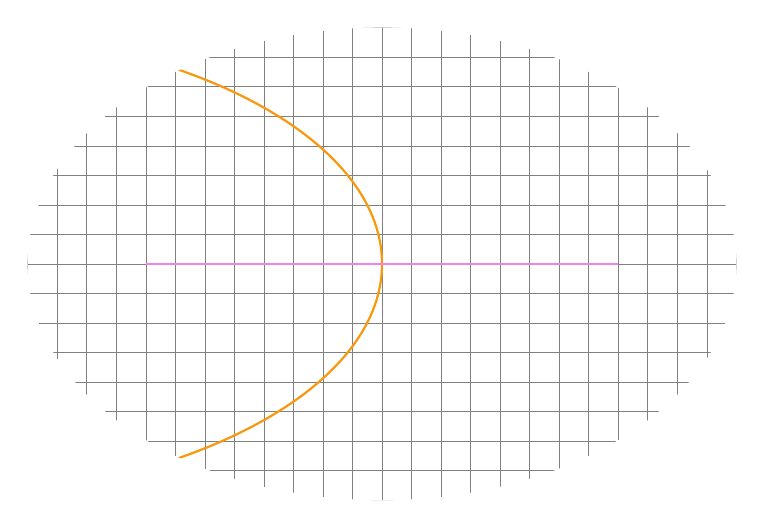
\begin{tikzpicture}[scale=3]
        \clip (1, 0) ellipse (1.5 and 1);
        \draw[step=.125, very thin, gray] (-2, -2) grid (3, 2);
        \draw[thick, color=YellowOrange] (-1, -1) arc (-90:90:2 and 1);
        \draw[thick, color=Violet] (0, 0) -- (2, 0);
    \end{tikzpicture}
\end{latex}

\subsection{Polar Coordinates}
We have been previously only using Cartesian Coordinates up until this point.
However, it may be convenient to represent information using Polar Coordinates in the future.

\begin{figure}[H]
    \centering
    \begin{tikzpicture}[scale=3]
        \draw (0, 0) -- (0.5, 0) arc (0:30:0.5) -- cycle;
        \draw (30:1cm) |- (0,0);
    \end{tikzpicture}
    \caption{Extended Angle}
    \label{fig:extendedangle}
\end{figure}

\begin{latex}
\begin{tikzpicture}[scale=3]
    \draw (0, 0) -- (0.5, 0) arc (0:30:0.5) -- cycle;
    \draw (30:1cm) |- (0,0);
\end{tikzpicture}
\end{latex}

Note how we easily extended the angle using Polar Coordinates.
Also note the new ``|-'' syntax which asks TikZ to draw a vertical line through the first argument intersection a horizontal line through the second argument.
We will condense more new syntax this way in the future as it does add completely new tools to our asenal but is good to know for niche situations such as the above.

\subsection{Relative Coordinates}
By default, Cartesian Coordinates are scaled to the previously defined vector, with $\begin{pmatrix} 1\\ 1\end{pmatrix}$ being the default vector.
We can ask for TikZ to draw points \textit{relative} to the previous vector using the +, ++ syntax

\begin{figure}[H]
    \centering
    \tikz \draw (0, 0) -- +(1, 2) -- +(3, 4) -- cycle;
    \caption{Basic Relative Coordintes}
    \label{fig:basicrelativecoordinates}
\end{figure}

\begin{latex}
    \tikz \draw (0, 0) -- +(1, 2) -- +(3, 4) -- cycle;
\end{latex}

\begin{figure}[H]
    \centering
    \tikz \draw (0, 0) -- ++(1, 2) -- ++(3, 4) -- cycle;
    \caption{Set Relative Coordintes}
    \label{fig:setrelativecoordinates}
\end{figure}

\begin{latex}
    \tikz \draw (0, 0) -- ++(1, 2) -- ++(3, 4) -- cycle; 
\end{latex}

Note the difference between the two, the ``+'' syntax is a scalar addition to the previous vector but does \textbf{not} mutate the previous vector in any way.
On the other hand, ``++'' has the same value as ``+'' but also mutates the previous vector to be the point to specified with the ``++'' syntax.

Both are plausible and no one is superior to the other in all cases.
We advise you to know your entire toolbox and choose the correct coordinate system when the time is right.

\subsection{Arrows}
\begin{figure}[H]
    \centering
    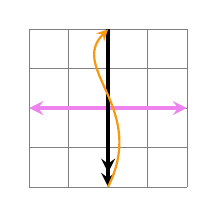
\begin{tikzpicture}[>=stealth]
        \draw[step=.5,color=gray,very thin] (-1, -1) grid (1, 1);
        \draw[<->, very thick, Violet] (-1, 0) -- (1, 0);
        \draw[<<-, very thick] (0, -1) -- (0, 1);
        \draw[->, thick, YellowOrange] (0, -1) .. controls (0.5, 0) and (-0.5, 0.5) .. (0, 1);
    \end{tikzpicture}
    \caption{Simple Arrow}
    \label{fig:simplearrow}
\end{figure}

\begin{latex}
    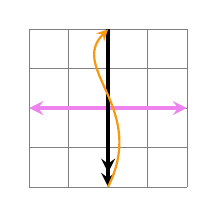
\begin{tikzpicture}[>=stealth]
        \draw[step=.5,color=gray,very thin] (-1, -1) grid (1, 1);
        \draw[<->, very thick, Violet] (-1, 0) -- (1, 0);
        \draw[<<-, very thick] (0, -1) -- (0, 1);
        \draw[->, thick, YellowOrange] (0, -1) .. controls (0.5, 0) and (-0.5, 0.5) .. (0, 1);
    \end{tikzpicture}
\end{latex}

As a rule of thumb, we can only draw arrows on paths that are open in some sense.
Note that we can indicate the kind of array head desired using the ``$>$'' option in the environent setting.


\newpage
\section{Options}
\subsection{Styles}
We now go on a slight detour.
If you came from any sort of programming background, you would know the important of avoiding code duplication.
TikZ gives us the ability to avoid passing the same options to the ``draw'' command by definiting ``styles''.

\begin{figure}[H]
    \centering
    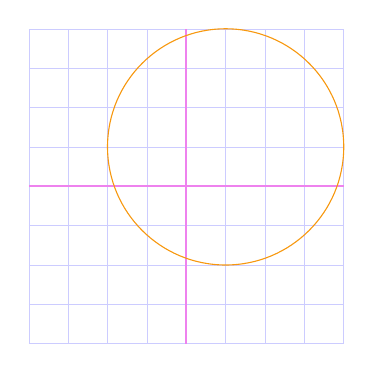
\begin{tikzpicture}
        \draw[step=.5, color=white!80!blue, very thin] (-2, -2) grid (2, 2);
        \draw[thick, color=Violet] (-2, 0) -- (2, 0);
        \draw[thick, color=Violet] (0, -2) -- (0, 2);
        \draw[color=YellowOrange] (0.5, 0.5) circle (1.5);
    \end{tikzpicture}
    \caption{Basic Styles}
    \label{fig:basicstyles}
\end{figure}

\begin{latex}
    \draw[step=.5, color=white!80!blue, very thin] (-2, -2) grid (2, 2);
    \draw[thick, color=Violet] (-2, 0) -- (2, 0);
    \draw[thick, color=Violet] (0, -2) -- (0, 2);
    \draw[color=YellowOrange] (0.5, 0.5) circle (1.5);
\end{latex}

The below is equivalent code, but much more extensible and modular.
\begin{latex}
    \tikzstyle Grid Line=[step=.5, color=white!80!blue, very thin]
    \tikzstyle Axis Line=[thick, color=Violet]
    \tikzstyle Circle Line=[color=YellowOrange]

    \draw[style=Grid Line] (-2, -2) grid (2, 2);
    \draw[style=Axis Line] (-2, 0) -- (2, 0);
    \draw[Axis Line] (0, -2) -- (0, 2);
    \draw[Circle Line] (0.5, 0.5) circle (1.5);
\end{latex}

Note that the ``style='' is optional.

One option we have is to compose and define styles with other styles.
If you have taken some form of an Object Oriented Programming course, we are employing Composition to avoid code repetition.
\begin{figure}[H]
    \centering
    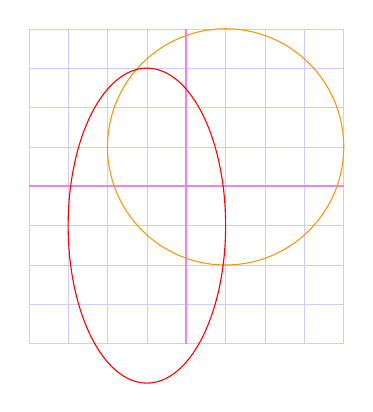
\begin{tikzpicture}
        \tikzstyle Grid Line=[step=.5, color=white!80!blue, very thin]
        \tikzstyle Axis Line=[thick, color=Violet]
        \tikzstyle Circle Line=[color=YellowOrange]

        \tikzstyle Ellipse Line=[Circle Line, color=Red]

        \draw[style=Grid Line] (-2, -2) grid (2, 2);
        \draw[style=Axis Line] (-2, 0) -- (2, 0);
        \draw[Axis Line] (0, -2) -- (0, 2);
        \draw[Circle Line] (0.5, 0.5) circle (1.5);
        \draw[Ellipse Line] (-0.5, -0.5) ellipse (1 and 2);
    \end{tikzpicture}
    \caption{Modified Style}
    \label{fig:modifiedstyle}
\end{figure}

\begin{latex}
    \tikzstyle Grid Line=[step=.5, color=white!80!blue, very thin]
    \tikzstyle Axis Line=[thick, color=Violet]
    \tikzstyle Circle Line=[color=YellowOrange]

    \tikzstyle Ellipse Line=[Circle Line, color=Red]

    \draw[style=Grid Line] (-2, -2) grid (2, 2);
    \draw[style=Axis Line] (-2, 0) -- (2, 0);
    \draw[Axis Line] (0, -2) -- (0, 2);
    \draw[Circle Line] (0.5, 0.5) circle (1.5);
    \draw[Ellipse Line] (-0.5, -0.5) ellipse (1 and 2);
\end{latex}

\subsection{Thickness}
We have already seen ``very thin'' in latex, Here are examples of other thickness of paths we can give to the draw command.
Note that ``thin'' gives us the default thickness.

\begin{figure}[H]
    \centering
    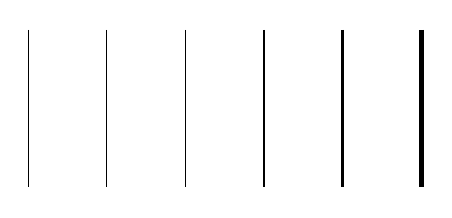
\begin{tikzpicture}
        \draw[ultra thin] (-2, 1) -- (-2, -1);
        \draw[very thin] (-1, 1) -- (-1, -1);
        \draw[thin] (0, 1) -- (0, -1);
        \draw[thick] (1, 1) -- (1, -1);
        \draw[very thick] (2, 1) -- (2, -1);
        \draw[ultra thick] (3, 1) -- (3, -1);
    \end{tikzpicture}
    \caption{Thickness}
    \label{fig:thickness}
\end{figure}

\begin{latex}
    \draw[ultra thin] (-2, 1) -- (-2, -1);
    \draw[very thin] (-1, 1) -- (-1, -1);
    \draw[thin] (0, 1) -- (0, -1);
    \draw[thick] (1, 1) -- (1, -1);
    \draw[very thick] (2, 1) -- (2, -1);
    \draw[ultra thick] (3, 1) -- (3, -1);
\end{latex}

\subsection{Scaling}
\begin{figure}[H]
    \centering
    \tikz \draw (0,0) circle (0.5);
    \caption{Small Circle}
    \label{fig:smallcircle}
\end{figure}

\begin{latex}
    \tikz \draw (0,0) circle (0.5);
\end{latex}

Suppose we want to enlarge the rendering without changing all the source code manually.
We can do so with the environment option ``scale''.

\begin{figure}[H]
    \centering
    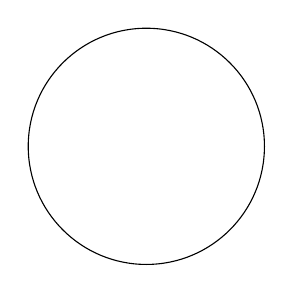
\begin{tikzpicture}[scale=3]
        \draw (0,0) circle (0.5);
    \end{tikzpicture}
    \caption{Scaled Circle}
    \label{fig:scaledcircle}
\end{figure}

\begin{latex}
    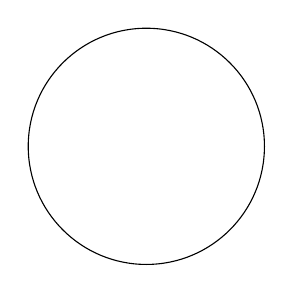
\begin{tikzpicture}[scale=3]
        \draw (0,0) circle (0.5);
    \end{tikzpicture}
\end{latex}

\subsection{Scoping}
We have previously been applying environment settings only to the ``tikzpicture'' environment, but what if we wanted for example to only change arrow head for a subset of the environment.
This can be accomplished with scopes

\begin{figure}[H]
    \centering
    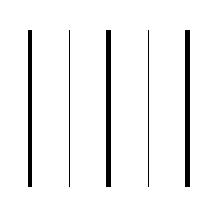
\begin{tikzpicture}[ultra thick]
        \draw(-1, -1) -- (-1, 1);
        \draw(0, -1) -- (0, 1);
        \draw(1, -1) -- (1, 1);
        \begin{scope}[ultra thin]
            \draw (-0.5, -1) -- (-0.5, 1);
            \draw (0.5, -1) -- (0.5, 1);
        \end{scope}
    \end{tikzpicture}
    \caption{Basic Scoped Lines}
    \label{fig:basicscopedlines}
\end{figure}

\begin{latex}
    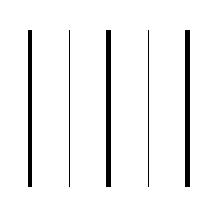
\begin{tikzpicture}[ultra thick]
        \draw(-1, -1) -- (-1, 1);
        \draw(0, -1) -- (0, 1);
        \draw(1, -1) -- (1, 1);
        \begin{scope}[ultra thin]
            \draw (-0.5, -1) -- (-0.5, 1);
            \draw (0.5, -1) -- (0.5, 1);
        \end{scope}
    \end{tikzpicture}
\end{latex}


\end{document}


